\begin{filecontents*}{\jobname.xmpdata}
  \Title{Software metrics in long-term projects}
  \Author{Santeri Suitiala}
  \Keywords{software\sep metrics\sep software quality}
  \Publisher{Aalto University}
\end{filecontents*}
\documentclass[oneside,pdfa]{aaltoseries}
\makeatletter
\@ifpackageloaded{inputenc}{%
  \inputencoding{utf8}}{%
  \usepackage[utf8]{inputenc}}
\hypersetup{hidelinks}                % Linkkien korostus pois
\makeatother
\usepackage[finnish,english]{babel}   % Kieli on englanti, tiivistelmässä suomi
\usepackage{setspace}                 % Rivivälin säätämiseksi
\usepackage{afterpage}                % Sivun taustaväri
\usepackage{apacite}		  % Bibtex
\usepackage{lastpage}
\microtypesetup{letterspace=25}       % Kannen harvaan välistykseen

\author{Santeri Suitiala}
\title{Software metrics in long-term projects}

\begin{document}


%%  KANSI  ---------------------------------------------

\thispagestyle{empty}
\setcounter{page}{0}  % Kansisivulle sivunumero 0

% Kansisivun marginaalit
\newgeometry{left=23.2mm,right=23.2mm,top=13.5mm,bottom=18mm}

%\pagecolor{white}\afterpage{\nopagecolor}
%{\color{black}  % Musta teksti

{\parindent0pt % Kappaleiden sisennys pois päältä
{\fontsize{11.9pt}{11.9pt}\bfseries\sffamily\lsstyle Bachelor’s Programme in Science and Technology}

%\color{white}  % Valkoinen teksti alkaa

\vspace{13.1mm}

\begin{spacing}{3.1}
{\fontsize{35}{35}\selectfont Software metrics in\\long-term projects}
\end{spacing}

\vspace{2.2mm}

\begin{spacing}{1.24}
{\fontsize{14pt}{14pt}\bfseries\sffamily\lsstyle Utilization and deployment of software metrics in long-lasting software projects}
\end{spacing}

\vspace{7.2mm}

\rule{\textwidth}{1.25pt}

\vspace{8.5mm}

{\fontsize{13.9pt}{13.9pt}\bfseries\sffamily\lsstyle Santeri Suitiala}

\vfill

\begin{picture}(0,0)
\put(356,-7.8){\bfseries\sffamily\footnotesize\lsstyle BACHELOR'S}
\put(356,-17.4){\bfseries\sffamily\footnotesize\lsstyle THESIS}
\put(346,-26.5){\rule{.75pt}{25pt}}
\end{picture}

\AaltoLogoSmall{.66}{?}{white}

} % Kappaleiden sisennys takaisin käyttöön
%} % Valkoisen tekstin pääätös



%%  NIMIÖSIVU  -----------------------------------------

\newpage

\pagenumbering{roman}

% Nimiösivun marginaalit
\newgeometry{left=80.7mm,right=25mm,top=12.9mm,bottom=21mm}

\thispagestyle{empty}

{\parindent0pt % Kappaleiden sisennys pois päältä
\begin{spacing}{1.1}
\hspace{-39.1mm}{\fontsize{10.5pt}{10.5pt}\sffamily\lsstyle Aalto University}

\hspace{-39.1mm}{\fontsize{10.5pt}{10.5pt}\bfseries\sffamily\lsstyle BACHELOR'S THESIS} {\sffamily\lsstyle 2018}
\end{spacing}

\vspace{12.7mm}

\begin{spacing}{1.63}
{\fontsize{17.8pt}{17.8pt}\selectfont Software metrics in long-life projects}
\end{spacing}

\vspace{10.5mm}

\begin{spacing}{1.2}
{\fontsize{13pt}{13pt}\selectfont Utilization and deployment of software metrics in long-lasting software project}
\end{spacing}

\vspace{10.6mm}

{\fontsize{13.9pt}{13.9pt}\bfseries\sffamily\lsstyle Santeri Suitiala}

\vfill

{\fontsize{10.3pt}{10.3pt}\sffamily\lsstyle\raggedright
\begin{spacing}{1.06}

Thesis submitted in partial fulfillment of the requirements for the
degree of Bachelor of Science in Technology.

Otaniemi, \today

\begin{tabbing}
Supervisor (ABB):\hspace{6mm} \= Jorma Keronen \\
Supervisor (Aalto):\hspace{6mm} \= Marko Hinkkanen \\
Advisor: \> Markus Turunen
\end{tabbing}
\vspace{-4mm}
\end{spacing}
} % fontsize

\vspace{11.5mm}

\begin{spacing}{.9}
{\bfseries\sffamily\lsstyle Aalto University \\
School of Electrical Engineering \\
Bachelor’s Programme in Science and Technology}
\end{spacing}
} % Kappaleiden sisennys takaisin käyttöön



%%  ABSTRACT  ------------------------------------------

\newpage
\phantomsection
\addcontentsline{toc}{chapter}{Abstract}

% Tiivistelmien marginaalit
\newgeometry{left=41.8mm,right=25mm,top=14.33mm,bottom=27mm}
% Alkuperäisessä Aalto-sarjassa marginaalit ovat suunnilleen näin:
%\newgeometry{left=41.8mm,right=17.6mm,top=14.33mm,bottom=20.4mm}

\begin{spacing}{.88}

{\parindent0pt % Kappaleiden sisennys pois päältä
\AaltoLogoSmall{.625}{''}{aaltoBlack}

{\fontsize{13.9pt}{13.9pt}\selectfont
\vspace{-8.9mm}\hfill{\bfseries\sffamily\lsstyle Abstract}}

{\fontsize{9.48pt}{9.48pt}\selectfont
\vspace{.9mm}\hfill{\bfseries\sffamily\lsstyle Aalto University, P.O. Box 11000, FI-00076 Aalto~~\textcolor{aaltoGray}{www.aalto.fi}}}

\vspace{7.8mm}{\fontsize{10.5pt}{10.5pt}\bfseries\sffamily\lsstyle Author}\\
{\small Santeri Suitiala}

\vspace{-2.4mm}\rule{\textwidth}{.75pt}

{\fontsize{10.5pt}{10.5pt}\bfseries\sffamily\lsstyle Title}\\
\parbox[t]{\textwidth}{\raggedright\small Software metrics in long-term projects}

\vspace{.5mm}\rule{\textwidth}{.75pt}

{\fontsize{10.5pt}{10.5pt}\bfseries\sffamily\lsstyle School}~~{\small School of Electrical Engineering}

\vspace{-2.4mm}\rule{\textwidth}{.75pt}

{\fontsize{10.5pt}{10.5pt}\bfseries\sffamily\lsstyle Degree programme}~~{\small Bachelor’s Programme in Science and Technology}

\vspace{-2.4mm}\rule{\textwidth}{.75pt}

{\fontsize{10.5pt}{10.5pt}\bfseries\sffamily\lsstyle Major}~~{\small Electronics and Electrical Engineering}\hfill{\fontsize{10.5pt}{10.5pt}\bfseries\sffamily\lsstyle Code}~~{\small ????}

\vspace{-2.4mm}\rule{\textwidth}{.75pt}

{\fontsize{10.5pt}{10.5pt}\bfseries\sffamily\lsstyle Supervisor (ABB)}~~{\small Jorma Keronen}

\vspace{-2.4mm}\rule{\textwidth}{.75pt}

{\fontsize{10.5pt}{10.5pt}\bfseries\sffamily\lsstyle Supervisor (Aalto)}~~{\small Marko Hinkkanen}

\vspace{-2.4mm}\rule{\textwidth}{.75pt}

{\fontsize{10.5pt}{10.5pt}\bfseries\sffamily\lsstyle Advisor}~~{\small Markus Turunen}

\vspace{-2.4mm}\rule{\textwidth}{.75pt}

{\fontsize{10.5pt}{10.5pt}\bfseries\sffamily\lsstyle Level}~~{\small Bachelor's thesis}\hfill{\fontsize{10.5pt}{10.5pt}\bfseries\sffamily\lsstyle Date}~~{\small \today}\hfill{\fontsize{10.5pt}{10.5pt}\bfseries\sffamily\lsstyle Pages}~~{\small \pageref{LastPage}}\hfill{\fontsize{10.5pt}{10.5pt}\bfseries\sffamily\lsstyle Language}~~{\small English}

\vspace{-2.4mm}\rule{\textwidth}{.75pt}

\vspace{6mm}

} % Kappaleiden sisennys takaisin käyttöön
\end{spacing}
\begin{spacing}{1.05}

\noindent{\fontsize{10.5pt}{10.5pt}\bfseries\sffamily\lsstyle Abstract}
\vspace{.8mm}

{\small
  Lorem ipsum.
}

\vfill

\end{spacing}
\begin{spacing}{.88}
{\parindent0pt % Kappaleiden sisennys pois päältä

\makebox[19mm][l]{\fontsize{10.5pt}{10.5pt}\bfseries\sffamily\lsstyle Keywords}\parbox[t]{123.6mm}{\raggedright\small software metrics, software quality}

\vspace{.5mm}\rule{\textwidth}{.75pt}

{\fontsize{10.5pt}{10.5pt}\bfseries\sffamily\lsstyle urn}~~{\small https://aaltodoc.aalto.fi}

\vspace{-2.4mm}\rule{\textwidth}{.75pt}

} % Kappaleiden sisennys takaisin käyttöön
\end{spacing}



\begin{spacing}{1.05}

\noindent{\fontsize{10.5pt}{10.5pt}\bfseries\sffamily\lsstyle Tiivistelmä}
\vspace{.8mm}

{\small
  Lorem ipsum.
}

\vfill

\end{spacing}
\begin{spacing}{.88}
{\parindent0pt % Kappaleiden sisennys pois päältä

\makebox[21mm][l]{\fontsize{10.5pt}{10.5pt}\bfseries\sffamily\lsstyle Avainsanat}\parbox[t]{121.6mm}{\raggedright\small ohjelmistometriikat, ohjelmiston laatu}

\vspace{.5mm}\rule{\textwidth}{.75pt}

{\fontsize{10.5pt}{10.5pt}\bfseries\sffamily\lsstyle urn}~~{\small https://aaltodoc.aalto.fi}

\vspace{-2.4mm}\rule{\textwidth}{.75pt}

} % Kappaleiden sisennys takaisin käyttöön
\end{spacing}

\selectlanguage{english}  % Palataan englantiin
\restoregeometry  % Palataan normaaleihin sivumarginaaleihin



%%  SISÄLTÖ  -------------------------------------------

\newpage

\tableofcontents

%%  TYÖ ALKAA TÄSTÄ  -----------------------------------

\newpage

\pagenumbering{arabic}


%% INTRODUCTION
\chapter{Introduction}

“The notion of ‘software engineering’ was first proposed in 1968” \cite{sommerville2011software}. Ever since the profession started, software projects have become bigger and more complex. This is because the hardware has been growing even faster and so software engineers have been having a hard time keeping the increasing phase up \cite{brooks1987no}. The increasing code complexity raises new problems with understanding existing code and increases probability of software flaws. Software complexity can be later decreased by refactoring code. Refactoring can mean e.g. removing duplicate code by abstracting, renaming and commenting the code to make it more readable.

Software metric is a quantitative value calculated from a piece of a code, a whole software project or even from a software process. Software metrics are used to track software code and process attributes to determine whether the software has improved or not. This thesis focuses on static product metrics. Knowing the change of the software quality over time makes it possible to plan and allocate resources to fix software with poor quality.

ABB Drives manufactures industrial drives which are controlled by software. Industrial drives are made to last for a long period of time and the same goes for the software inside the machine. Also new bugs are found and customers demand new features which makes the software evolve rapidly over time. The same effect that Brooks discovered over 30 years ago is something that still exists in companies: software size and complexity increases over time. Without refactoring, the software may become ambiguous and useless for the developers.  If too much time is spent refactoring and improving the code, no new feature gets developed and customers are left unsatisfied. In a big company, it is difficult to perceive the whole picture and so the golden mean of internal improving and feature development can be hard to find.

This thesis introduces the underlying theory of software metrics. Furthermore a part of the task is also to determine the core metrics by getting familiar with the most commonly used metrics, try selected metrics in the real world and make conclusions. Later this thesis tries to improve development process that the research and development department is using and guide the development teams to the right direction by introducing a systematic and automated daily software analysis. Analysis calculates different core software metrics and ideally represents a long-term graph to determine whether the quality and other attributes of the software is increasing or decreasing and how rapid is the change.

The ultimate goal of this thesis is to help the company’s software development teams to decide when to refactor code and improve tools and dependencies and how much time should be used for it.



%% CHAPTER 2
\chapter{Theory behind software metrics}

Software measurement is a quantitative value calculated from a software process or system. A software metric can either be a software measurement or a function of many different software measurements. Software metrics are used to track e.g software quality or cost estimation. Tracking the quality of software makes it easier and more efficient to see whether software system and process has improved or not. Knowing the direction of the software quality makes it possible to plan and give resources to fix software or process with poor quality or efficiency. 

\section{Classification of software metrics}

\begin{figure}[t!]
\centering
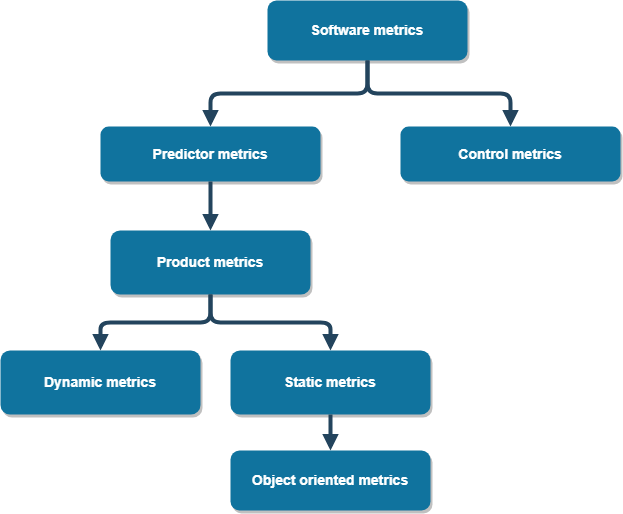
\includegraphics[scale=0.05]{metrictree.png}
\caption{Software metric types}
\label{fig:metrictree}
\end{figure}

Software metrics can be divided into product, process and project metrics. Project metrics \cite{dineshthakur}. Project metrics help project managers to estimate projects by tracking for example amount of developers or delivered lines of code. This helps to estimate similar projects in the future. Process metrics measures values concerning software development processes. Thakur lists e.g. number of error found before the software release and conformity to schedule to be process metrics. These metrics help project stakeholder to perceive how the project is proceeding.
Product metrics gives measurements from the developed software product \cite{sommerville2011software}.  A simple example of a process metric is source lines of code (SLOC) which simply tells the number of lines of code the whole program has altogether \cite{nguyen2007sloc}. Figure~\ref{fig:metrictree} tries to present and to help understand the division of different kind of software metrics. This thesis focuses on product metrics. 

\subsection{Product metrics}

Many defined sets of product metrics exists. One defined set is e.g Halstead metrics \cite{al2005analysis}. It is also possible to adjust an existing metric for specified software or implement a completely new metric. A product metric can either be dynamic or static \cite{sommerville2011software}. Dynamic metrics are measured when a program is executing and static metrics can be measured e.g by reading the source code or documentation of a program. This thesis focuses on static code analysis. Dynamic metric such as server uptime is easy to interpret as 100\% would be the wanted outcome. Static metrics has the problem that those can often be unambiguous and easily to be misinterpreted. For example SLOC can be 5000 in one product and one million in other. That doesn't mean that other is better quality software than the other. 

The magnitude of the metric does not matter. We are more interested about the change of the metric over a defined amount of time. Other approaching method for product metrics is comparing different results inside the project that is being analyzed. If a part of a software project has anomalous attributes, it should be investigated further. 

\subsection{Traditional and object-oriented metrics}

Traditional metrics can be calculated from any kind of software. Traditional product metrics are for example SLOC and cyclomatic complexity \cite{fenton1997software}.

\section{Halstead complexity measures}

Lorem ipsum.




%% CHAPTER 3
\chapter{Determining useful metrics}

Determining the right software is not always a simple task. Measurements can be ambiguous due to the fact that the measurement outputs are just numbers. These number's real correlation to the software quality may be easy to misinterpret.

\section{Software metrics in agile development process}

The software development team that is the target of this thesis is using an agile software development process. Agile methods are 

\section{Source code examples}
To really test if the metrics are correlating software quality we need to first determine low and high quality source code examples. These examples should be good or bad quality code according to the whole development teams opinion. After we have determined what good and bad quality concretely means we can start to figure out which metrics correlate to the quality. 

\section{Trial and error approach}


%% CHAPTER 4
\chapter{Implementing analysis for a development team}

After we are sure that the software metrics really are useful and capable of indicating software quality it is time to make use of the metrics. In this chapter a proof of concept will be implemented and possibly introduced for the software development team's use.

\section{Essential tools for implementation}

For a concrete implementation, some software tools are needed. The preference is that metrics are easily visible and understandable for each developer. Metrics are not meant to be a stressing factor which might happen if the metrics are forced to be seen on a day-to-day basis. Metrics should rather be an auxiliary tool to help developers perceive a bigger picture regarding source code. No comparison was done while choosing the tools and the main idea is to use tools that are easily available or already in use by the company.

\subsection{Software analysis tool}

CppDepend\footnote{https://www.cppdepend.com/} is a commercial tool specifically made to analyze C/C++ code. It provides many of the common software metrics and has a good-looking user interface. There are many other promising tools but investigating available options is out of scope on this thesis. Using this tool gives a good indication if software metrics are useful for the software development team or not. If the tool later turns out to be exchangeable with a more usable one, it can easily be replaced.

\subsection{Analysis automation tool}

Jenkins\footnote{https://jenkins.io/} is an open-source continuous integration tool. Jenkins is a server that can easily be set to trigger for example CppDepend to analyze source code daily. It can also be set to store artifacts which in this case would be the analysis outcome in Hypertext Markup Language (HTML) format.  The strength of Jenkins is that anyone in the research and development department who has access to the internet can observe the outcome of the analysis. Source code is updated to the latest version with the help of Git\footnote{https://git-scm.com/}. Git is a distributed version control system that is widely used by globally \cite{gitsurvey}.

\subsection{Build server}

Analysis can not be done on any computer. It must be a computer that is constantly powered on and online. For this purpose a build server will be set up. Jenkins will be connected to this computer and will tell it to do the required commands.

\section{System description}

\begin{figure}[t!]
\centering
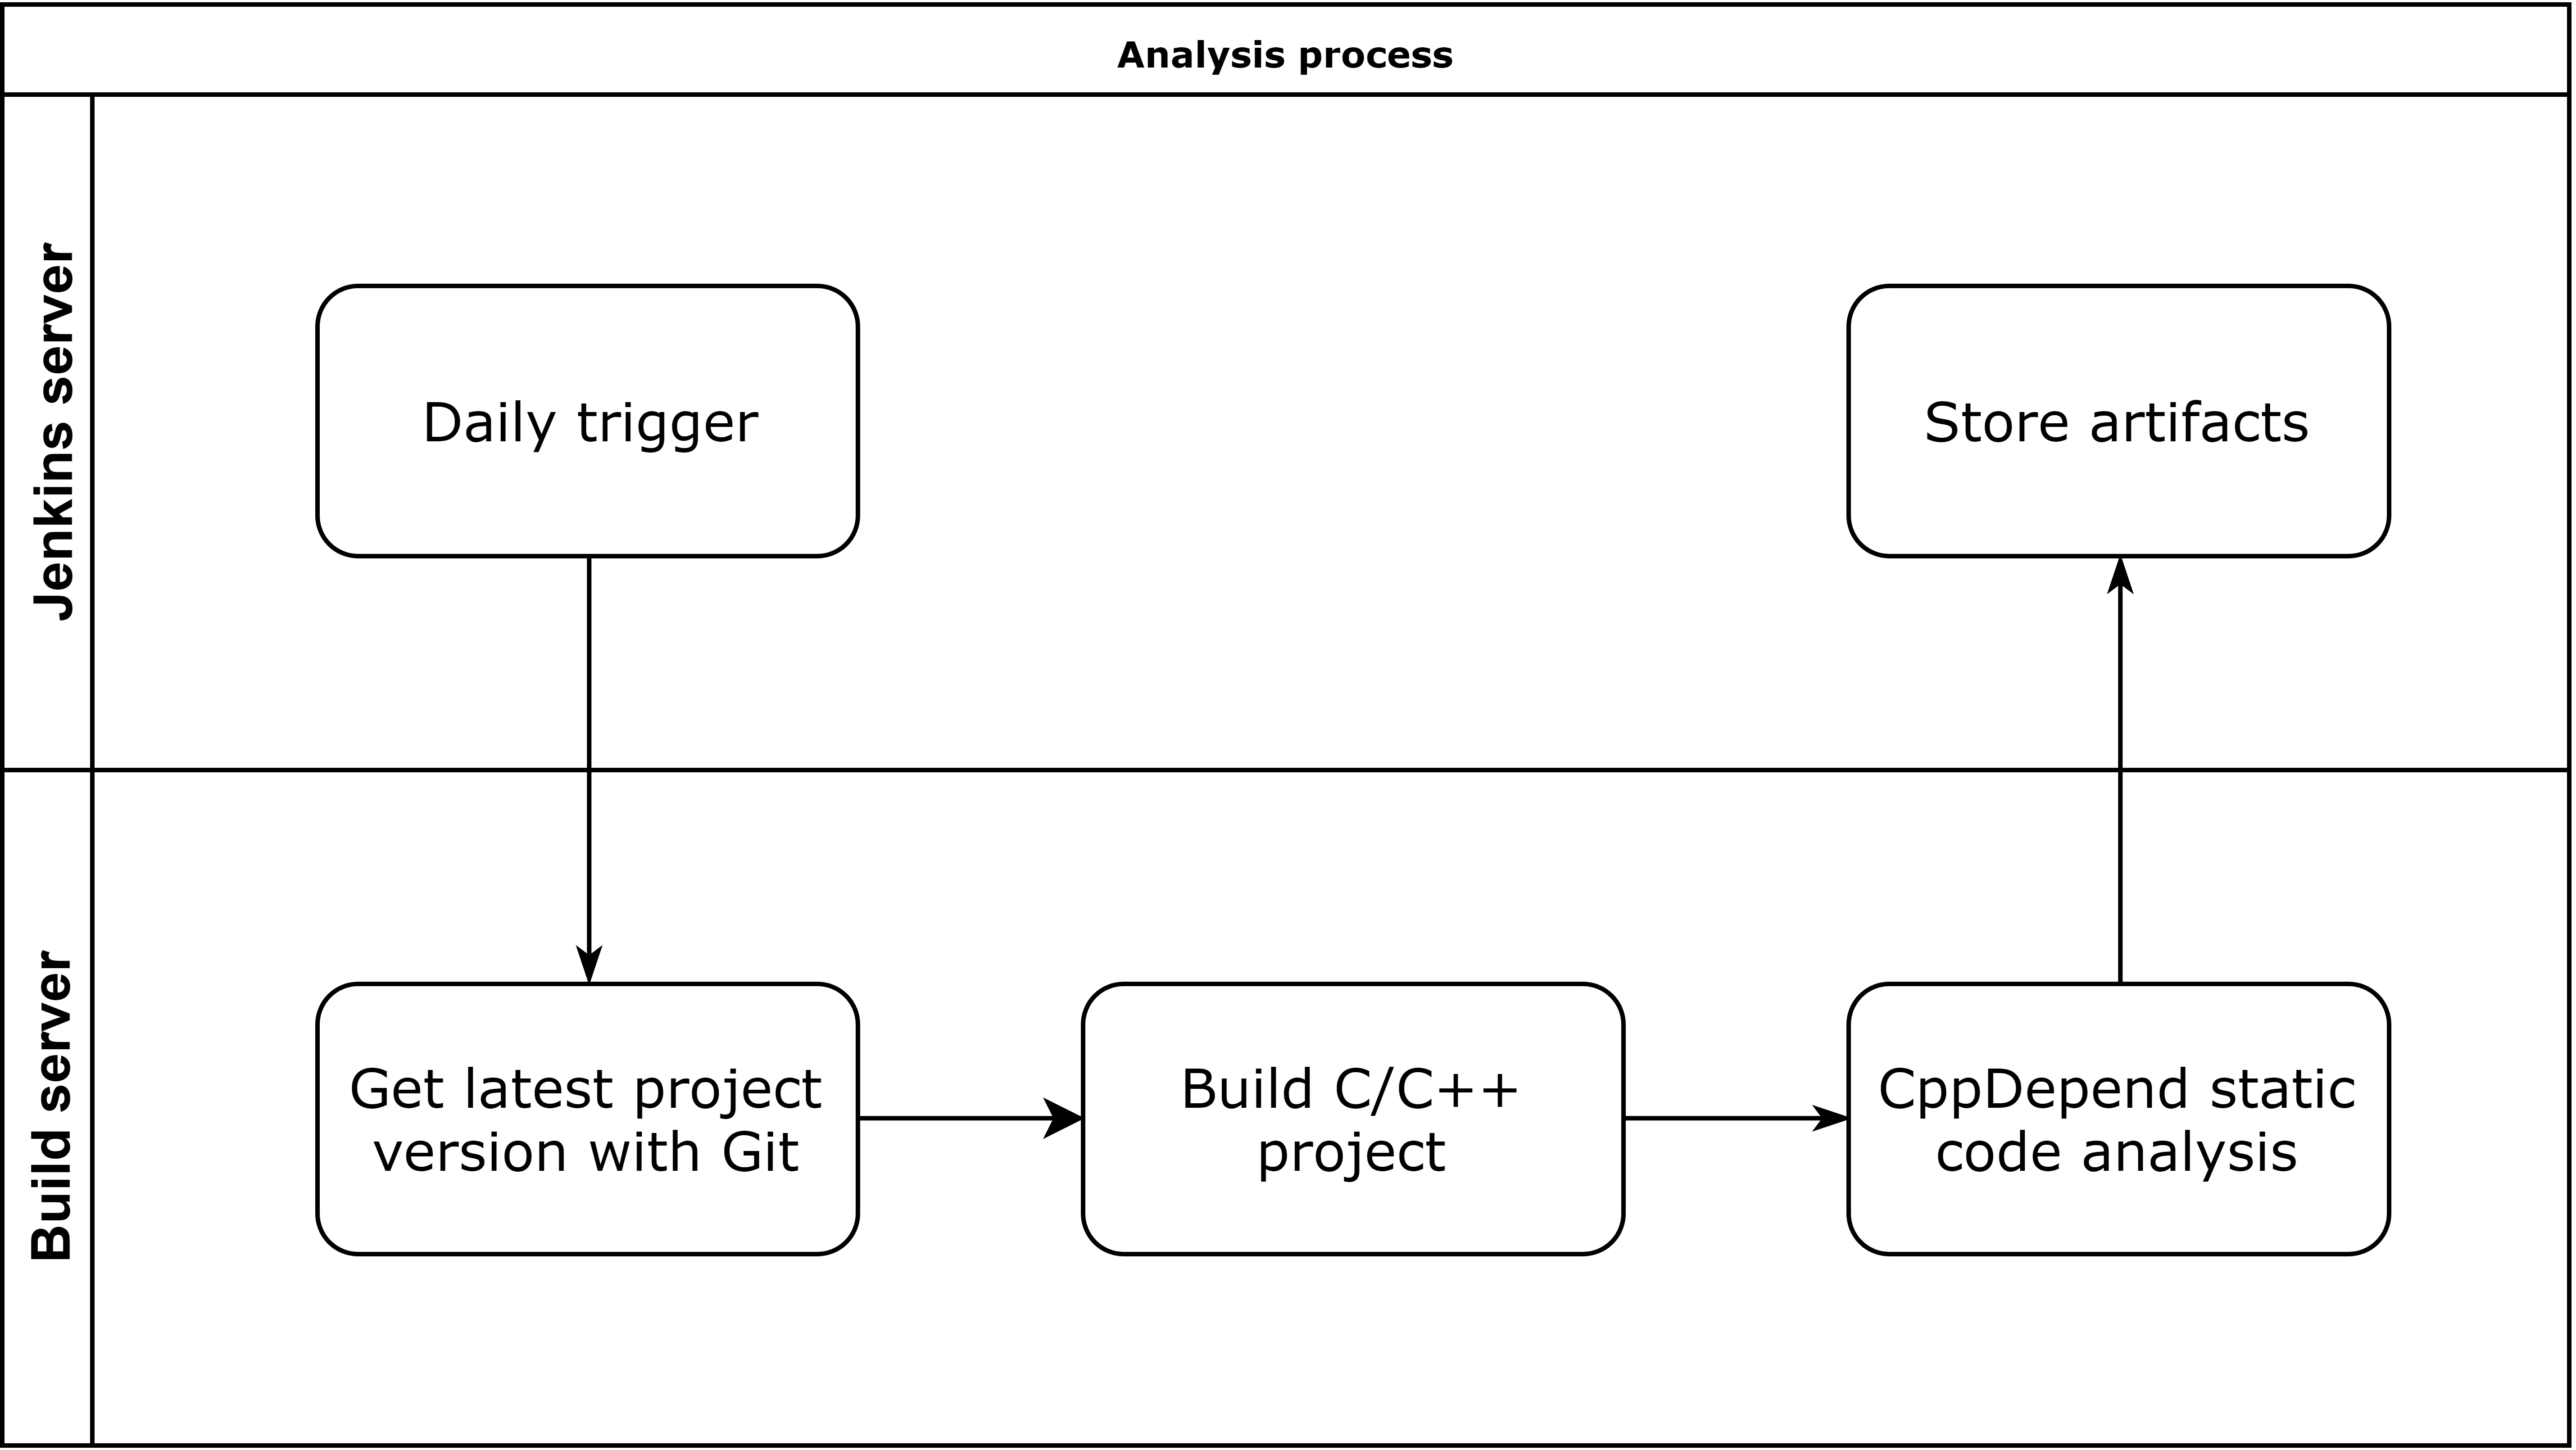
\includegraphics[scale=0.06]{systemdesc.png}
\caption{System funcionality}
\label{fig:systemdesc}
\end{figure}

The selected tools will form a system that will create desired analysis daily to our Jenkins server where it can be inspected by everyone. The system functionality is illustrated in figure~\ref{fig:systemdesc}. 

%% 5 CHAPTERS TOO MUCH?
\chapter{Conclusions}

Lorem ipsum.

%%  LIITTEET  ------------------------------------------

\bibliographystyle{apacite}
\bibliography{references}

\end{document}
